\chapter{Combinatory Engine}
    \section{Descripci\'on del Problema}\label{descripcionproblema}
        El desarrollo del motor combinatorio, a partir de este momento ser\'a denominado \combeng, se vio originado por la necesidad de \fudepan \
        (Fundaci\'on para el Desarrollo de la Programaci\'on en \'Acidos Nucleicos) de contar con uno. En dicha fundaci\'on se presentan de ma\-ne\-ra
        recurrente, problemas de car\'acter bioinform\'atico. Una familia de ellos se ve caracterizada por compartir una o m\'as de las siguientes
        caracter\'isticas:
        \begin{itemize}
            \item Requerir un motor combinatorio para la generaci\'on de \'arboles de combinaciones.
            \item Utilizar mecanismos de poda sobre dichos \'arboles.
            \item Requerir un sistema de puntuaci\'on por cada una de las combinaciones (\textit{ranking} o \textit{scoring}).
        \end{itemize}

		El principal objetivo de este proyecto fue el de acoplar a \fud \ una capa que permita, a usuarios sin altos conocimientos en programaci\'on, 
		implementar soluciones a los problemas antes mencionados.

		La elecci\'on de acoplar \combeng \ como una nueva capa del framework \fud \ en lugar de crear un proyecto aparte, se debi\'o a que la mayor\'ia de los 
    problemas antes mencionados requieren un elevado nivel de c\'omputo, muchas veces ``\textit{imposible}'' de realizar en una \'unica computadora.

  \newpage
	\section{Nuevas Capas De FuD}
		A continuaci\'on, puede observarse un nuevo diagrama, al estilo OSI de redes, reemplazando al diagrama inicial del framework \fud \ 
		mostrando las diferentes capas:
    \begin{figure}[H] \hspace{.30cm}
        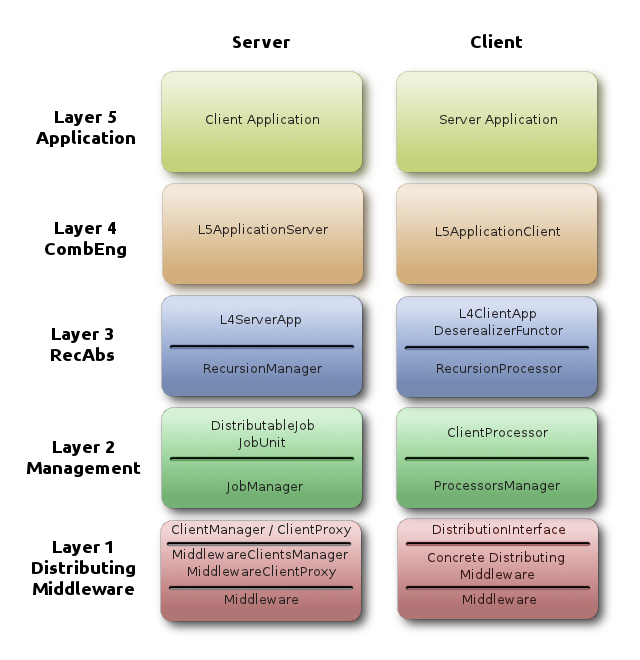
\includegraphics[scale=.51]{images/AbstractLayersRedesigned.png}
	         \caption{Vista abstracta de las nuevas capas en una instancia de uso de \fud}
	         \label{redisenioFud}
    \end{figure}
		
    Claramente se puede observar la existencia de otra nueva capa, denominada \recabs
    \footnote{\url{http://code.google.com/p/fud/source/browse/branches/FuD-duplex/layers/layer3-recabs/}}. La misma constituye otro proyecto de la
    fundaci\'on y es con el que \combeng \ interact\'ua, por lo que a continuaci\'on se explica en qu\'e consiste el mismo.
		
		\section{RecAbs}
			\recabs, al igual que el presente trabajo, surge como una propuesta de \fudepan. En tal fundaci\'on se necesitaba una biblioteca que facilitara
      la soluci\'on a un gran n\'umero de proyectos bioinform\'aticos, los cuales usan a la recursi\'on como mecanismo fundamental y poseen muchos
      factores de implementaci\'on en com\'un.

      La meta de este proyecto es identificar una abstracci\'on gen\'erica con una estructura com\'un a todas las soluciones recursivas a estos
      problemas de inter\'es y, al mismo tiempo, proveer una soluci\'on algor\'itmicamente eficiente para dichos proyectos. Esta abstracci\'on abarca
      la familia de problemas que cumplen las siguientes condiciones:

      \begin{itemize}
        \item la soluci\'on se adapte a un modelo recursivo. No obstante, se ajusta principalmente a aquellos problemas con definici\'on 
          inherentemente recursiva; y 
        \item los nodos del \'arbol de recursi\'on de la soluci\'on sean (horizontalmente) independientes.
      \end{itemize}

      Cabe destacar que, cualquiera sea el problema que se desee resolver por medio de \recabs, debe adoptar la forma recursiva, donde el paso
      inductivo conduce a problemas cada vez mas peque\~nos que, necesariamente, terminar\'an en, por lo menos, un caso base. Tambi\'en es
      significativo el segundo punto, el cual expresa que s\'olo se pueden solucionar problemas con la recursividad m\'as simple, es decir, 
      una vez llegado a las hojas esa ejecuci\'on se da por terminada y se informa un resultado, es imposible volver a pasos anteriores buscando
      diferentes caminos, como si lo permiten algoritmos de backtracking, combinatorios, etc.
			
			\subsection{Arquitectura}
				Dado que \recabs \ tambi\'en forma parte del framework, presenta el modelo cliente-servidor. El Servidor tiene la responsabilidad de iniciar 
				el proceso recursivo, administrar los pasos de recursi\'on que realizan los clientes y llevar el control de los resultados, mientras que el 
        cliente es el encargado de la resoluci\'on de un \textit{functor recursivo} (ver \ref{recursiveFunctor}). Durante la tarea de resoluci\'on, 
        el cliente puede pedir ayuda y solicitar el env\'io tanto de functores intermedios como de resultados al servidor.
				
				\recabs \ es un proyecto bastante extenso, por lo que s\'olo se har\'a menci\'on a aquellos componentes que interact\'uan de manera directa con 
				\combeng, es decir, aquellas interfaces de L3 que poseen servicios o funcionalidades a ser implementadas por capas superiores.
				
        \subsubsection{Lado Servidor}
					\begin{description}
            \item \textit{RecursionManager}: Es el ``handler'' del lado servidor. Cada paquete que sale de un cliente y llega a este \textit{manager},
              puede ser alguno de los siguientes tipos de paquetes:
              \begin{itemize}
                \item un \textbf{resultado}, parcial y relativo a la unidad de trabajo que se proces\'o, el cual es tratado de la manera que el usuario
                  desee. Indica, en el cliente, que se ha llegado a una hoja en el \'arbol de recursi\'on.
                \item un \textbf{mensaje intermedio} es cualquier dato transmitido de cliente a servidor sin llegar a una hoja o estado final en el
                  \'arbol, y por lo tanto no es un resultado. Tambi\'en es enviado (en cliente) y tratado (en servidor) como el usuario disponga.
                \item una \textbf{unidad de trabajo} a distribuir, la cu\'al ser\'a enviada a un cliente ocioso. Un \textit{trabajo} arribado es una
                  partici\'on del trabajo del cliente que lo envi\'o. 
              \end{itemize}
              Otro rol fundamental que juega el \textit{manager} es la de iniciar el proyecto implementado sobre \recabs. Para ello, el mismo cuenta
              con la ayuda de \textit{L4ServerApp} que nos brinda el functor inicial, el cual es apilado para distribuirlo al primer cliente ocioso
              que se encuentre, donde as\'i la iniciaci\'on del proceso recursivo.
						\item \textit{L4ServerApp}: La implementaci\'on de esta interfaz consta de los siguientes puntos:
              \begin{itemize}
                \item brindar el \textit{functor} inicial,
                \item definir qu\'e har\'a con los resultados a medida que lleguen, y
                \item definir el tratamiento de los mensajes intermedios (si es que los hubiera).
              \end{itemize}
              De estos requisitos, el primero es obligatorio mientras que los otros dos restantes son opcionales en la medida que la aplicaci\'on
              arroje resultados y mensajes intermedios.
					\end{description}

          \subsubsection{Lado Cliente}
					\begin{description}
						\item \textit{RecursiveProcessor}: Es el encargado de realizar la ejecuci\'on total (o parcial) del functor que fue asignado a un cliente.
						\item \textit{DeserializerFunctor}:	Provee los servicios de transformaci\'on de un paquete serializado a un functor recursivo.
            \item \textit{DistributionPolicy}: Es una interfaz que ofrece varios ``sabores'' de distribuci\'on ya implementados, as\'i como la posibilidad de
              extender este conjunto de pol\'iticas si el desarrollador quisiese. Cada pol\'itica establece cu\'ando un cliente debe distribuir o
              cu\'ando debe parar y, en caso positivo, cu\'anto debe distribuir. Cuando se menciona \textit{distribuir}, se hace referencia al env\'io 
              de unidades de trabajo a clientes ociosos que el server dispone.
					\end{description}

          \subsubsection{Com\'un a Ambos Lados}
					\begin{description}
            \item \textit{RecursiveFunctor}\label{recursiveFunctor}: es una abstracci\'on a la \textit{funci\'on recursiva} de una aplicaci\'on \recabs.
              Una aplicaci\'on deber\'a implementar la interfaz definida por \texttt{RecursiveFunctor}, este nuevo \textit{functor} (por ejemplo, 
              \texttt{ConcreteFunctor}) representar\'a la funci\'on que el usuario desee distribuir. Estos nuevos functores encapsulan la informaci\'on 
              espec\'ifica de cada aplicaci\'on, la cual es necesaria y suficiente para ser procesada por los clientes.
						\item \textit{SerializableRecursiveFunctor}: Es un RecursiveFunctor para proyectos distribuidos, por lo que agrega el servicio de 
						serializaci\'on.
					\end{description}
		
    \section{?`Qu\'e es CombEng?}
    	Como se mencion\'o anteriormente, \combeng \ constituye una capa de un framework para la implementaci\'on de aplicaciones distribuidas. Define una 
    	interfaz clara y sencilla para que un usuario pueda implementar sus aplicaciones independiz\'andose de todas aquellas tareas involucradas en computaci\'on 
    	distribuida, como la divisi\'on del trabajo, la administraci\'on de los clientes que realizan el procesamiento, la recolecci\'on de los resultados, etc.
        
		\combeng \ no depende del problema a ser implementado, sino que define una estructura com\'un para implementar aquellos problemas que compartan las 
		caracter\'isticas mencionadas en \ref{descripcionproblema}. La soluci\'on al problema constituir\'a una nueva capa, por encima de L4, la cual recibe el nombre 
		de \textit{Application Layer}

    \section{?`C\'omo Funciona Un Proyecto \combeng?}
        \combeng \ esta dividido en dos aplicaciones: \textit{Cliente} y \textit{Servidor}. Luego, durante la ejecuci\'on de cualquier proyecto
        \combeng, deber\'a existir exactamente un \'unico servidor y cualquier n\'umero de clientes conectados al mismo. El servidor y sus clientes se
        relacionan de modo Master-Worker, en el sentido de que el servidor (Master) es el encargado de llevar a cabo el progreso general del sistema
        y los clientes (Workers) son los que hacen el procesamiento de datos.
        
        Para comprender c\'omo se lleva a cabo el procedimiento se introduce a continuaci\'on, la terminolog\'ia del proyecto.
        \subsection{El Nodo}\label{nodoL4}
            \texttt{L4Node} es un concepto abstracto de \textit{estado} de una aplicaci\'on \combeng. Una aplicaci\'on tendr\'a que implementar la interfaz 
            definida por \texttt{L4Node} (por ejemplo, \texttt{L5Node}). Estos nuevos nodos tienen la responsabilidad de encapsular la informaci\'on de 
            inter\'es para la aplicaci\'on, disponer del conocimiento suficiente para procesar tal informaci\'on, establecer el progreso general de la
            ejecuci\'on, entre otras.

        \subsection{La Pol\'itica de Combinaci\'on}
            Una \textit{Pol\'itica de Combinaci\'on} define el modo en que una colecci\'on de elementos debe ser combinada. \combeng \ provee un conjunto de estas 
            pol\'iticas y las hay en dos sabores, \textit{simples} y \textit{compuestas}. De todas formas, el desarrollador de una aplicaci\'on puede crearse 
            tantas como sea necesario, s\'olo debe respetar las interfaces que L4 le impone. Las pol\'iticas compuestas establecen el comportamiento de dos o m\'as
            pol\'iticas simples. Para m\'as detalles, ver \ref{composedCombinationPolicies}.
            
        \subsection{La Pol\'itica de Poda}
            Una \textit{Pol\'itica de Poda} establece reglas que permiten acotar el espacio de b\'usqueda en un \'arbol de ejecuci\'on. Este tipo de pol\'iticas 
            puede influenciar tanto en la performance como en el tiempo de ejecuci\'on de una aplicaci\'on. Cabe notar que en la mayor\'ia de estas
            aplicaciones, los espacios de b\'usqueda son de gran tama\~no.

        \subsection{La Aplicaci\'on Servidor}
            \texttt{L5ApplicationServer} es, como su nombre lo indica, la aplicaci\'on del lado servidor. Esta aplicaci\'on es la encargada de iniciar todo el
            proceso y, para \'ello, necesita del nodo inicial (ra\'iz del \'arbol de ejecuci\'on) junto con la colecci\'on de datos sobre la cual operar\'a el 
            motor combinatorio. Adem\'as, desempe\~na la tarea de recolectar y procesar los resultados que los clientes le env\'ian.
            
            En cap\'itulos posteriores se introducen algunas \textit{application layers}, reflejando con m\'as claridad las nociones de nodo/estado, 
            colecci\'on inicial de elementos para el motor combinatorio, y dem\'as.
            
        \subsection{La Aplicaci\'on Cliente}
			\texttt{L5ApplicationClient} es la aplicaci\'on del lado cliente y es la encargada de procesar la informaci\'on contenida en el nodo que el servidor 
			le ha asignado. 
			
			Si bien el usuario desconoce c\'omo se lleva a cabo la distribuci\'on del trabajo en las capas inferiores del framework, aqu\'i resulta de gran 
      inter\'es por lo que se realiza una breve descripci\'on de ello\footnote{Para m\'as informaci\'on, consulte \textit{RecAbs}
      (\url{http://code.google.com/p/fud/source/browse/branches/FuD-duplex/layers/layer3-recabs/})}.
			
			Como se mencion\'o anteriormente, \texttt{L5ApplicationServer} es el que inicia todo el proceso. Luego, a grandes rasgos, el comportamiento de
      un cliente puede ser resumido en los siguientes pasos:
      \begin{enumerate}
        \item Recibe, del servidor, un nodo para procesar.
        \item Se obtienen todos los estados posteriores (los nodos hijos de aquel que fue recibido).
        \item Enviar informaci\'on al servidor (resultados) en caso de ser necesario.
        \item Continuar con el procesamiento de los nuevos nodos generados. Para ello, se consulta al servidor qu\'e hacer:
          \begin{enumerate}
            \item Si el servidor dispone de otros clientes conectados, el cliente corriente delegar\'a tantos nodos como sea posible.
            \item Caso contrario, \'el mismo continuar\'a con el proceso de ejecuci\'on.
          \end{enumerate}
        \item Una vez finalizada la tarea encomendada por el servidor, notifica al mismo de tal situaci\'on y queda a la espera de un nuevo trabajo.
      \end{enumerate}

\newpage
    \section{Dependencias Externas}
		Adem\'as de las bibliotecas STL (Standard Template Library) de C++, \combeng \ depende de otra biblioteca muy importante, que se enuncia a continuaci\'on.
		
		\subsection{MiLi}\label{mili}
		MiLi es una colecci\'on de peque\~nas bibliotecas C++, compuesta \'unicamente por \textit{headers}. Sin necesidad de instalaci\'on, sin un \textit
    {makefile}, sin complicaciones. Soluciones simples para problemas sencillos.
		
		Esta biblioteca provee varias funcionalidades peque\~nas en archivos cabecera (m\'as conocidos en el \'ambito de C/C++, extensi\'on ``.h''), 
    y puede ser descargada junto con su documentaci\'on desde el siguiente enlace\\ \url{http://mili.googlecode.com/}.
		
		MiLi ha sido utilizada extensamente a lo largo del desarrollo de \combeng \ donde, particularmente, se destacan las funcionalidades provistas por 
		\textit{binary-streams} y \textit{container-utils}.
		\begin{itemize}
			\item \textbf{binary-streams:} esta biblioteca permite empaquetar diferentes tipos de datos dentro de un \'unico objeto usando operadores de
        stream (\textless\textless \ y \textgreater\textgreater). En la Tabla \ref{bstreamusage} se muestra un ejemplo de su uso.
			\item \textbf{container-utils:} esta biblioteca provee un conjunto de funciones, optimizadas para cada tipo de contenedor STL:
				\begin{itemize}
					\item \texttt{find(container, element)}.
					\item \texttt{find(container, element, nothrow)}.
					\item \texttt{contains(container, element)}.
					\item \texttt{insert\_into(container, element)}.
					\item \texttt{copy\_container(from, to)}.
				\end{itemize}
								
				Adicionalmente, esta biblioteca provee las siguientes clases:
				\begin{itemize}
					\item \texttt{ContainerAdapter<T>}
					\item \texttt{ContainerAdapterImpl<T, ContainerType>}
				\end{itemize}
				Estos \textit{container adapters} son una herramienta para lidiar con diferentes contenedores STL de manera homog\'enea, sin necesidad de conocer 
				el tipo de contenedor que es (vector, list, map, set). Los usuarios pueden invocar al m\'etodo \texttt{insert(const T\&)} para insertar un 
				elemento de tipo T sin la necesidad de saber el tipo del contenedor. En el Cuadro 4.1 se muestra un ejemplo de su uso.
		\end{itemize}
		
		\begin{table}[!htb]
        	\lstset{language=C++}
        	\begin{lstlisting}[frame=single]
#include <iostream>
#include <string>
#include <vector>
#include "include/mili.h"

int main()
{
    std::vector<int> v(5,3); //all 3's
    v[1] = 1;
    v[4] = 7; //so it is [3,1,3,3,7]

    bostream bos;
    bos << 1 << 2 << 3 << std::string("Hello ") << v << 4 << std::string("World!");

    bistream bis(bos.str());

    int         nums[4];
    std::string str1;
    std::string str2;

    std::vector<int> v2;


    bis >> nums[0] >> nums[1] >> nums[2] >> str1 >> v2 >> nums[3] >> str2;

    for (int i=0; i < 4 ; ++i)
        std::cout << nums[i] << std::endl;

    std::cout << str1 << str2 << std::endl;

    std::cout << '[';
    for (size_t i=0; i < 5; ++i)
        std::cout<< v2[i] << ' ';
    std::cout << ']' << std::endl;
}
        	\end{lstlisting}
        	\centering \caption{C\'odigo extra\'ido de Mili::binary\_streams.} 
        	\label{bstreamusage}
        \end{table}
        
        		\begin{table}[!htb]
        	\lstset{language=C++}
        	\begin{lstlisting}[frame=single]
#include <iostream>
#include <vector>
#include <string>
#include <queue>
#include "mili/mili.h"
using namespace std;

template <class T>
static void insert_elements(T& container);

int main()
{
    vector<int> v;
    v.push_back(1);
    map<string, string> m;
    m["hello"] = "good bye";
    m["Bonjour"] = "au revoir";
    m["hola"] = "adios";
    m["buenas"] = "adios";

    try
    {
        cout << contains(v, 2) << endl;         // will print 0 (false)
        cout << contains(m, "nothing") << endl; // will print 0

        cout << "map: " << endl;
        cout << remove_first_from(m, "au revoir") << endl; // will print 1
        cout << remove_all_from(m, "adios") << endl;  	   // will print 1

        cout << find(v, 1) << endl;         // will print 1 (true)
        cout << find(m, "hello") << endl;   // will print "good bye"
        cout << find(m, "world") << endl;   // will throw ElementNotFound
    }
    catch (ElementNotFound)
    {
        cerr << "Element not found!" << endl;
    }

    /* TEST - queue in container_utils::insert_into */
    queue<int> myqueue;
    insert_elements(myqueue);

    return 0;
}

template <class T>
static void insert_elements(T& container)
{
    insert_into(container, 100);
    insert_into(container, 100);
    insert_into(container, 100);
    insert_into(container, 200);
    insert_into(container, 300);
    insert_into(container, 400);
    insert_into(container, 400);
}
        	\end{lstlisting}
        	\centering \caption{C\'odigo extra\'ido de Mili::container\_utils.} 
        	\label{cointailerUtils}
        \end{table}

